\section{\textsc{Scrambled eggs on wholemeal rolls}}

\subsection*{Ingredients for 2 portions:}

\begin{tabular}{p{7.5cm} p{7.5cm}}
	& \\
	5 eggs & 2 wholemeal rolls \\
	1 tomato & 20g butter \\
  1tbsp cress & 2 salad leaves \\
  fresh herbs & tartar sauce \\
  oil for the pan & a sip of mineral water \\
  salt, pepper \& nutmeg
\end{tabular}

\subsection*{Serving suggestion:}

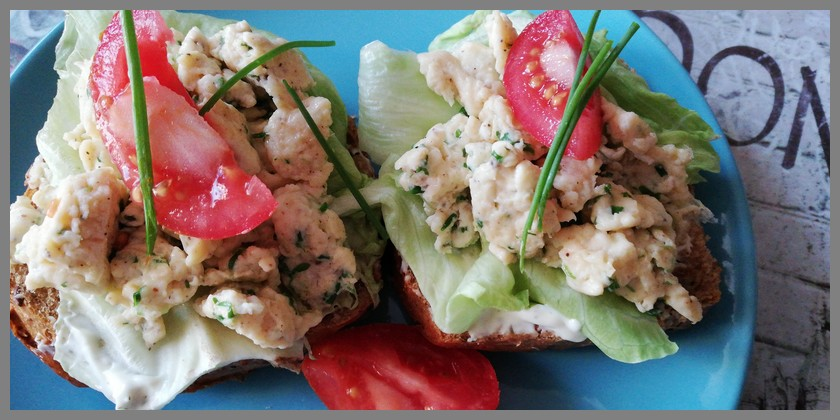
\includegraphics[width=\textwidth]{img/ruehrei_vollkorn.jpeg} \cite{ruehreivollkorn}

\subsection*{How it's done:}

\begin{tabular}{p{15cm}}
	\\
  Mix eggs, herbs and mineral water in a bowl.\\
  Heat the oil in a flat pan. Add the egg mass.\\
  Leave to falter and gradually slide from the outside to the inside with a scraper.\\
  In the meantime, cut the rolls open and coat them with tartar sauce.\\
  Place a salad leaf on top. Spread the scrambled eggs on the salad and garnish with half a tomato.
\end{tabular}
